\documentclass{beamer}

% uncomment to generate printer friendly scaled version
\usepackage{pgfpages}
\usepackage[utf8]{inputenc}
\usepackage[ngerman]{babel}
\usepackage[T1]{fontenc}
\usepackage{graphicx}


\usepackage{listings} \lstset{numbers=left, numberstyle=\tiny, numbersep=2pt, showstringspaces=false, basicstyle=\scriptsize} \lstset{language=Java} 

\usetheme{Darmstadt}
% BUILD SCRIPT HOOKS - DO NOT REMOVE THIS COMMENTS %
%%%%%THEME_PLACEHOLDER_JENKINSBUILD%%%%%
%%%%%HANDOUT_PLACEHOLDER_JENKINSBUILD%%%%%
% END OF BUILD SCRIPT HOOKS %
%\pgfpagesuselayout{4 on 1}[a4paper,border shrink=5mm,landscape]

\setbeamercovered{transparent}
%\setbeamertemplate{footline}[frame number]

\title{Test-driven development}
\subtitle{mit JUnit, Mockito und PowerMock}

\institute[TD 2k11]{Computerseminar Tondorf 2011}

\author[F. Becker, B. Neff]{
        Felix Becker \& 
	Benjamin Neff
}

\begin{document}

	\begin{frame}
		\titlepage
	\end{frame}

	\begin{frame}
		\frametitle{Agenda}
		\setcounter{tocdepth}{1}
		\tableofcontents
	\end{frame}
	
	%
	% Einfuehrung
	%

	\section{Einführung}
	
		\subsection{Einführung in Test-driven development}

			\begin{frame}
				\frametitle{Was ist Unit-Testing?}

				Unit-Testing ist toll!
			\end{frame}

			\begin{frame}
				\frametitle{Was ist Test-driven development?}

				Test-driven development ist toll!
			\end{frame}

	%
	% Tools und Frameworks
	%
	
	\section{Tools \& Frameworks}

		\subsection{Was gibt es für Tools und Frameworks?}

			\begin{frame}
				\frametitle{Frameworks}

				\begin{itemize}
					\item{JUnit}
					\item{Mockito}
					\item{PowerMock}
					\item{(TestNG)}
				\end{itemize}
			\end{frame}

			\begin{frame}
				\frametitle{Continuous Integration}

				\begin{itemize}
					\item{Hudson / Jenkins}
					\item{Continuum}
					\item{\ldots}
				\end{itemize}
			\end{frame}

			\begin{frame}
				\frametitle{EMMA}

				\begin{figure}[htb]
					\begin{center}
						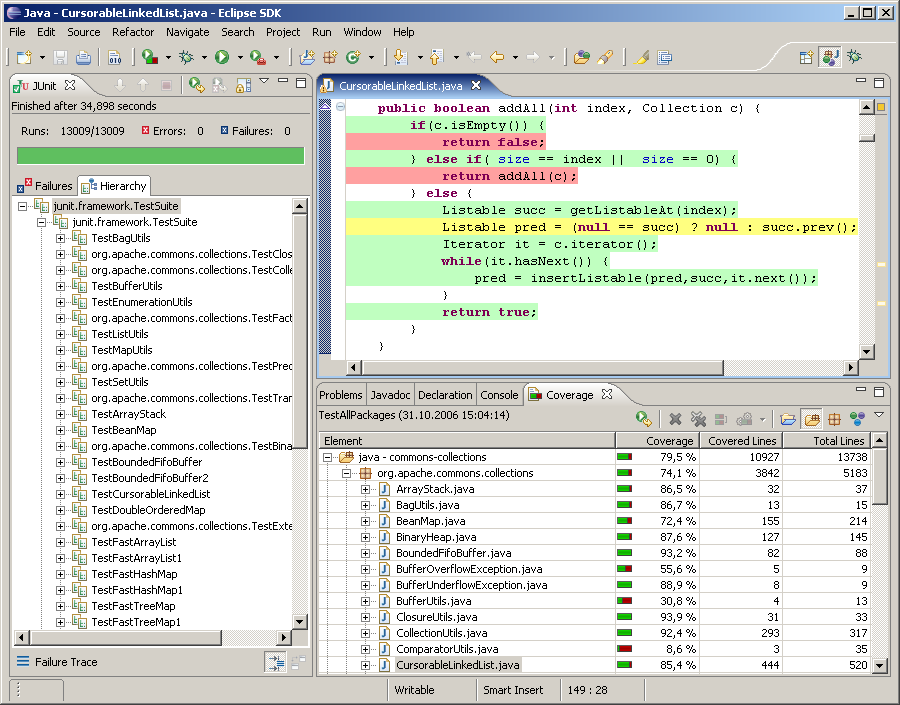
\includegraphics[scale=0.25]{eclemma}
					\end{center}
					\caption{http://www.eclemma.org/images/screen.png}
				\end{figure}
			\end{frame}

	%
	% JUnit und Mockito
	%
	
	\section{JUnit \& Mockito}

		\subsection{Testen mit JUnit}

			\begin{frame}
				\frametitle{Was ist JUnit?}

				\begin{itemize}
					\item{''Standard''-Framework für Java-Unittests}
					\item{Testergebnis OK (grün) / nicht OK (rot)}
					\item{Sehr einfache Bedienung (Annotations, \ldots)}
					\item{Aktuelle Version: JUnit 4}
				\end{itemize}
			\end{frame}

			\begin{frame}[fragile]
				\frametitle{Test-Klasse}

				\begin{lstlisting}
					public class CalculatorTest {
					  private Calculator calculator;

					  @Before
					  public void setup() {
					    calculator = new Calculator();
					  }

					  @Test
					  public void testSum(){
					    assertEquals(5, calculator.sum(2, 3));
					  }

					  @Test
					  public void testSumWithNegativeValue(){
					    assertEquals(-5, calculator.sum(-2, -3));
					  }
					  // ...
					}
				\end{lstlisting}
			\end{frame}
		
			\begin{frame}[fragile]
				\frametitle{Zu testende Beispielklasse}

				\begin{lstlisting}
					public class Calculator {
					  public int sum(int x, int y){
					    return x + y;
					  }
					  // ...
					}
				\end{lstlisting}
			\end{frame}

			\begin{frame}[fragile]
				\frametitle{Fehlerfall testen}

				\begin{lstlisting}
					@Test(expected = DivisionByZeroException.class)
					public void expectExceptionOnDivisionByZero(){
					  calculator.divide(1, 0);
					}
				\end{lstlisting}
			\end{frame}

		\subsection{Mocking mit Mockito}

			\begin{frame}
				\frametitle{Was ist ein Mock?}

				\begin{itemize}
					\item{engl. Mock-up (Attrappe / Simulation)}
					\item{Attrappe eines Objekts}
					\item{Selbe Schnittstelle wie das Original-Objekt}
					\item{Ersatz für Komponenten, die die zu testende Komponente benötigt}
					\item{Garantiert definiertes Verhalten während des Tests}
				\end{itemize}
			\end{frame}

			\begin{frame}
				\frametitle{Mockito}

				\begin{itemize}
					\item{Sehr einfache Mock-Erstellung}
					\item{Mockverhalten leicht konfigurierbar}
					\item{Aufzeichnung aller Mock-Calls}
					\item{Werkzeuge zur Verifikation von Mock-Calls}
				\end{itemize}
			\end{frame}

		%\subsection{Partial Mocking} frame wenn es eine mockito technologie ist

	%
	% PowerMock
	%
	
	\section{PowerMock}

		\subsection{Einleitung}

			\begin{frame}
				\frametitle{PowerMock}

				\begin{itemize}
					\item{Mit Java-Bordmitteln normalerweise nicht mockbare Komponenten mocken}
					\item{Deep and dark magic}
						\begin{itemize}
							\item{Byte code Manipulation (javaassist)}
							\item{Classloader-Manipulation}
						\end{itemize}
				\end{itemize}
			\end{frame}

		\subsection{Constructor call prevention}

			\begin{frame}[fragile]
				\frametitle{A constructor nightmare}

				\begin{lstlisting}
					public class Foo {
					  public Foo(){
					    if(!MyFrameworkMegaUtil.isFrameworkProperlyInitialized()){
					      MyFrameworkMegaUtil.initializeFramework();	
					    }
					  }

					  public int sum(int x, int y){
					    return x+y;
					  }
					}
				\end{lstlisting}
			\end{frame}

			\begin{frame}[fragile]
				\frametitle{Solution!}

				\begin{lstlisting}
					public class FooTest {
					  @Test
					  public void testSum(){
					    Foo comp = WhiteBox.newInstance(Foo.class);
					    assertEquals(5, comp.sum(2, 3));
					  }
					}
				\end{lstlisting}
			\end{frame}

		\subsection{Static / Final Mocks}

			\begin{frame}[fragile]
				\frametitle{A static nightmare}

				\begin{lstlisting}
					public class Foo {
					  public int testMe(){
					    int sth = sth();
					    int y = DrEvil.getEvil(sth);	
					    return sth + y;
					  }
					  // ...
					}

					public class DrEvil {
					  public static int getEvil(int x){
					    return doReallyEvilStuff();
					  }
					}
				\end{lstlisting}
			\end{frame}

			\begin{frame}[fragile]
				\frametitle{Solution!}

				\begin{lstlisting}
					@PrepareForTest(DrEvil.class)
					public class FooTest {
					  @Test
					  public void testIt(){
					    PowerMockito.mockStatic(DrEvil.class);
					    Mockito.when(DrEvil.getEvil(anyInt())).thenReturn(1);
					    Foo foo = new Foo();
					    assertEquals(1,foo.testMe());

					    // static verification
					    PowerMockito.verifyStatic();
					    DrEvil.getEvil(anyInt());
					  }
					}
				\end{lstlisting}
			\end{frame}


	%
	% Abschluss 
	%

	\section{Abschluss}

		\subsection{Common Pitfalls}

			\begin{frame}
				\frametitle{Beachten!}

				\begin{itemize}
					\item{Nicht die Implementierung sondern das Verhalten der Komponente testen (Refactoring von ungetestetem Code!)}
					\pause
					\item{Zu viele static-Mocks weisen auf Design-Probleme hin}
					\pause
					\item{Zu niedrige Code-Coverage nach Testfertigstellung weist auf ein Design-Problem hin (auch Boilerplate abdecken!)}
					\pause
					\item{Immer Fehlerfallverhalten der Komponente testen (Logging, Returnvalues, \ldots)}
					\pause
					\item{Zu ''lange'' Testfälle weisen auf ein Problem hin}
				\end{itemize}
			\end{frame}

		
		\subsection{Danke und Quellen}

			\begin{frame}
				Fragen? Nein? Danke!
			\end{frame}

			\begin{frame}
				\frametitle{Quellen und Wissenswertes}

				\scriptsize
				Wissenswertes
				\begin{itemize}
					\item{\url{http://de.wikipedia.org/wiki/Modultest}}
					\item{\url{http://de.wikipedia.org/wiki/Testgetriebene\_Entwicklung}}
					\item{\url{http://de.wikipedia.org/wiki/Mock-Objekt}}
				\end{itemize}

				JUnit \& Mockito \& PowerMock
				\begin{itemize}
					\item{JUnit: \url{http://www.junit.org}}
					\item{Mockito: \url{http://www.mockito.org}}
					\item{PowerMock: \url{http://code.google.com/p/powermock/}}
				\end{itemize}

				Hudson \& Jenkins \& EMMA
				\begin{itemize}
					\item{Hudson: \url{http://www.hudson-ci.org}}
					\item{Jenkins: \url{http://www.jenkins-ci.org}}
					\item{EMMA: \url{http://emma.sourceforge.net}}
					\item{Ecl-Emma: \url{http://www.eclemma.org}}
				\end{itemize}
			\end{frame}

\end{document}
